\label{sec:1d}
\subsection{Implementation}
The 1-dimensional models are run from \texttt{lab2p1.m} in Section
\ref{sec:lab2p1}. The models themselves are represented by the \texttt{OneD}
class from the \texttt{OneD.m} file in Section \ref{sec:oned}.

\subsection{Results}
Each data set yielded varying results with the different approximation methods.
The Gaussian samples, shown in Figures \ref{fig:gg}, \ref{fig:ge} and
\ref{fig:gu}, the parametric estimation assuming the unknown density is
Gaussian is closest to the original. For the exponential samples in Figures
\ref{fig:eg}, \ref{fig:ee} and \ref{fig:eu}, the
parametric estimation assuming theunknown density is exponential is closest to
the original.

The Parzen window method, depicted in Figures \ref{fig:parzen1} and \ref{fig:parzen4} does a
better estimation than the parametric methods when the model assumption does
not match the real distribution. This is due to the fact that Parzen windows do
not make assumptions about the distribution, they simply model the points that
they find. With a wider window such as in Figure \ref{fig:parzen4}, the estimated density
can be made smoother. However, trade-off is made between the smoothness of the estimated PDF and its
sensitivity to sample data.

It is not always possible to use a parametric approach. Parametric
approaches require estimation of the parameters using methods such as ML that
requires us to solve some equations. However, sometimes these equations could
be extremely difficult to solve if the PDF of the assumed distribution are not
in simple form. Besides, it is likely that the sample data do not follow any
known distributions, especially when the number of the sample data is very
small. Therefore, it is sometimes hard if not impossible to use a pararametric approach.

A parametric method is preferred if the sample data follows the assumed
distribution closely and the parameters can be easily computed. In contrast, a
non-parametric approach is preferable if the sample data do not follow any
particular known distribution or the number of samples are very small.

\begin{figure}
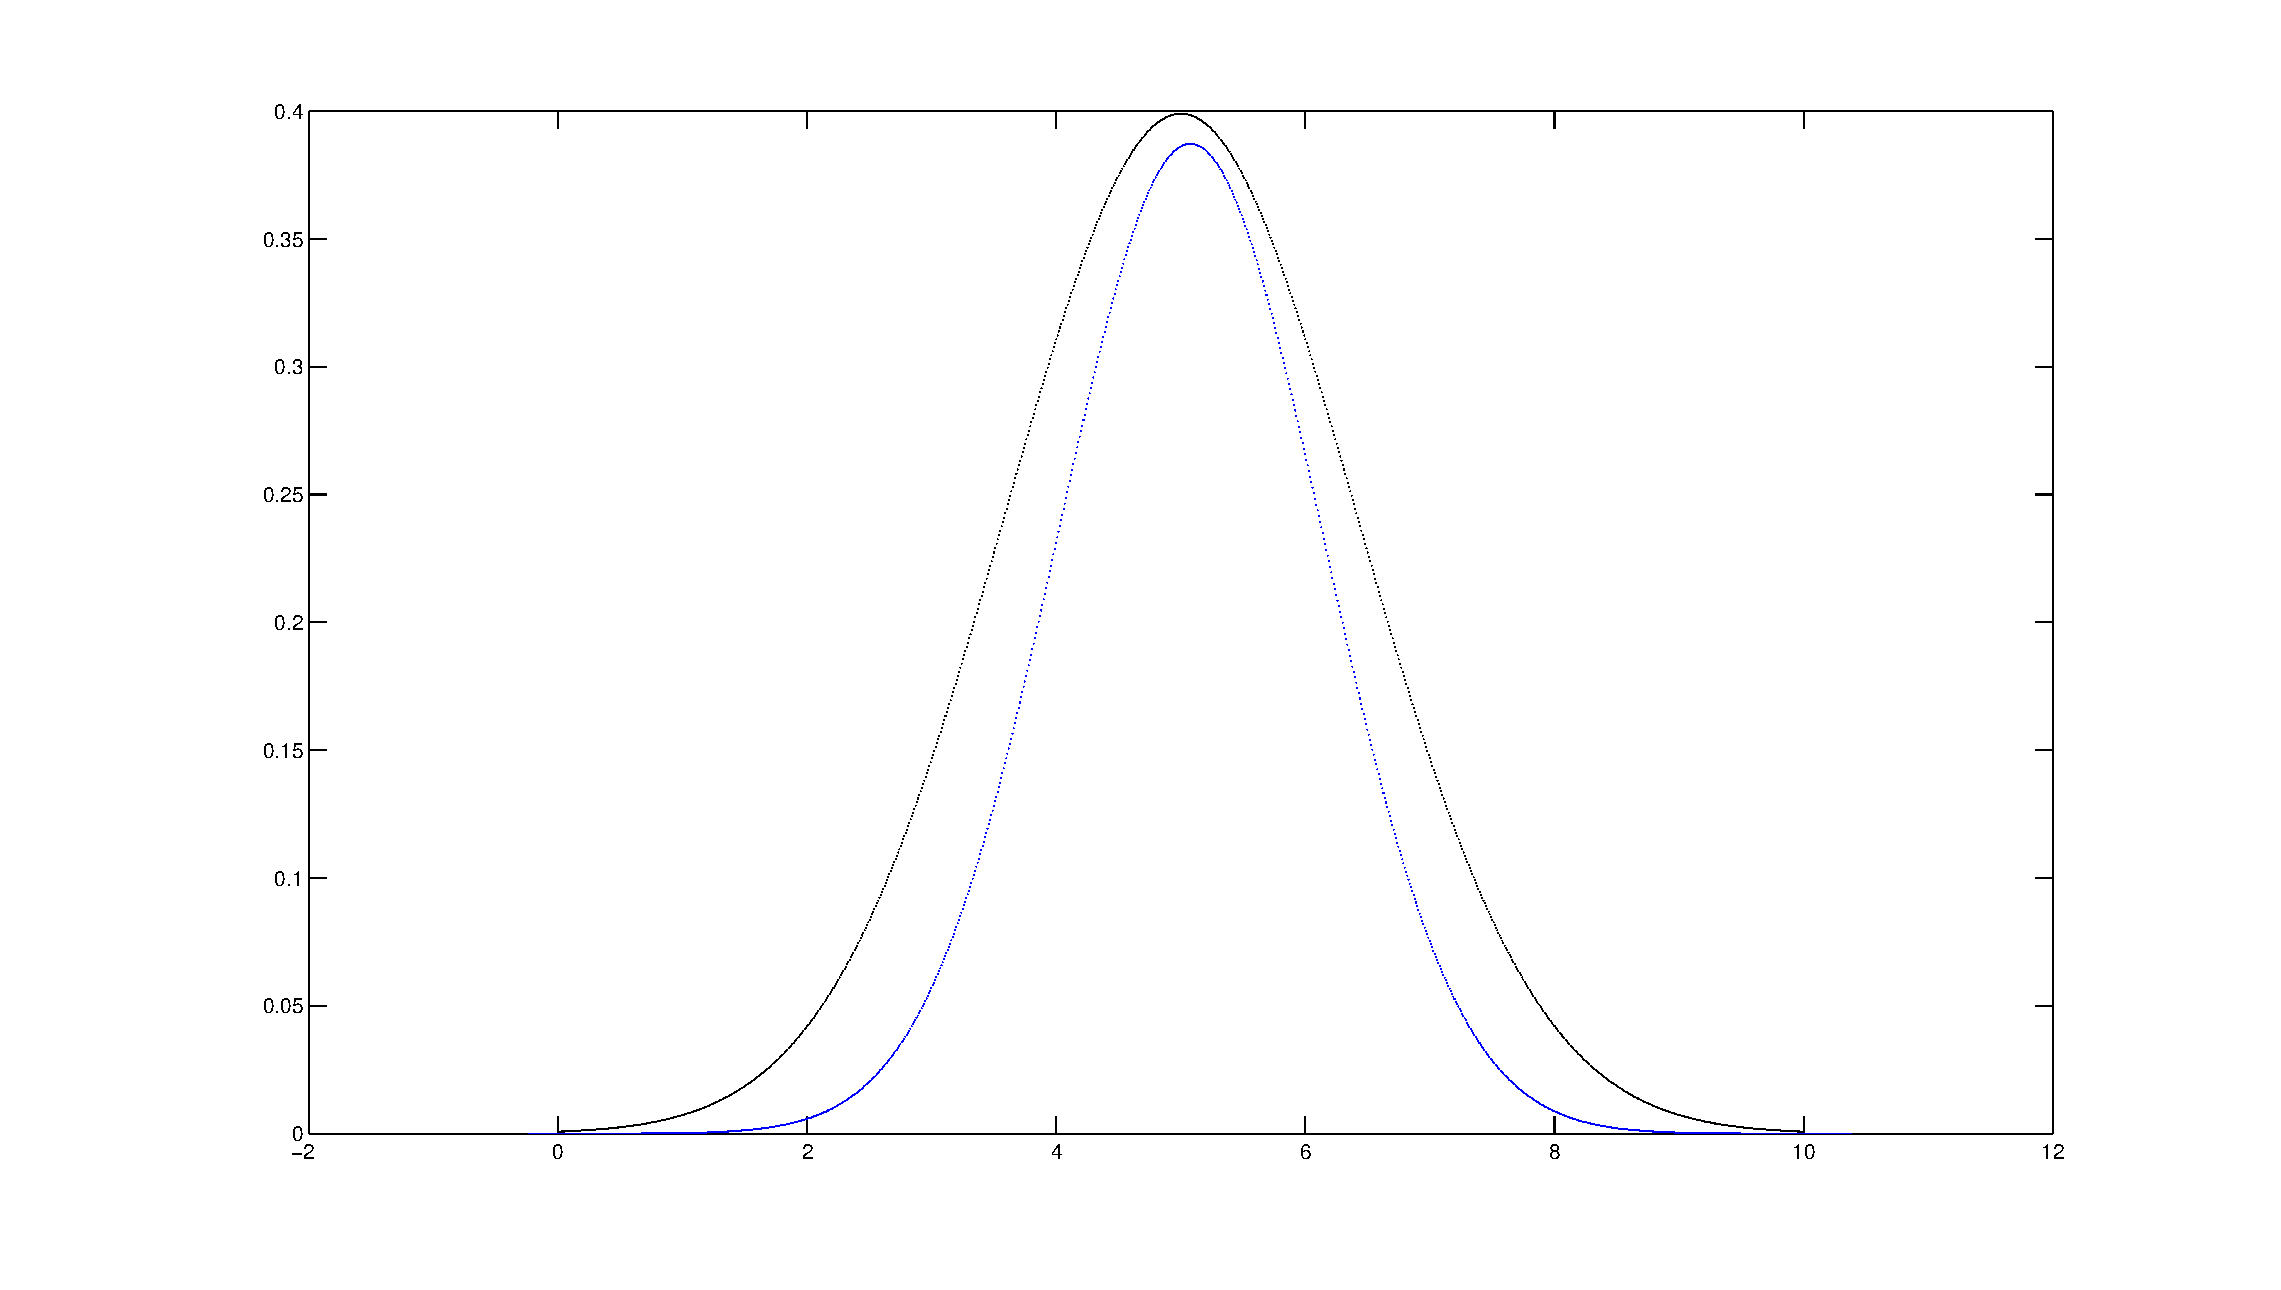
\includegraphics[scale=0.4]{gauss-gauss}
\caption{Gaussian sample (black) estimated assuming a Gaussian PDF (blue)}
\label{fig:gg}
\end{figure}

\begin{figure}
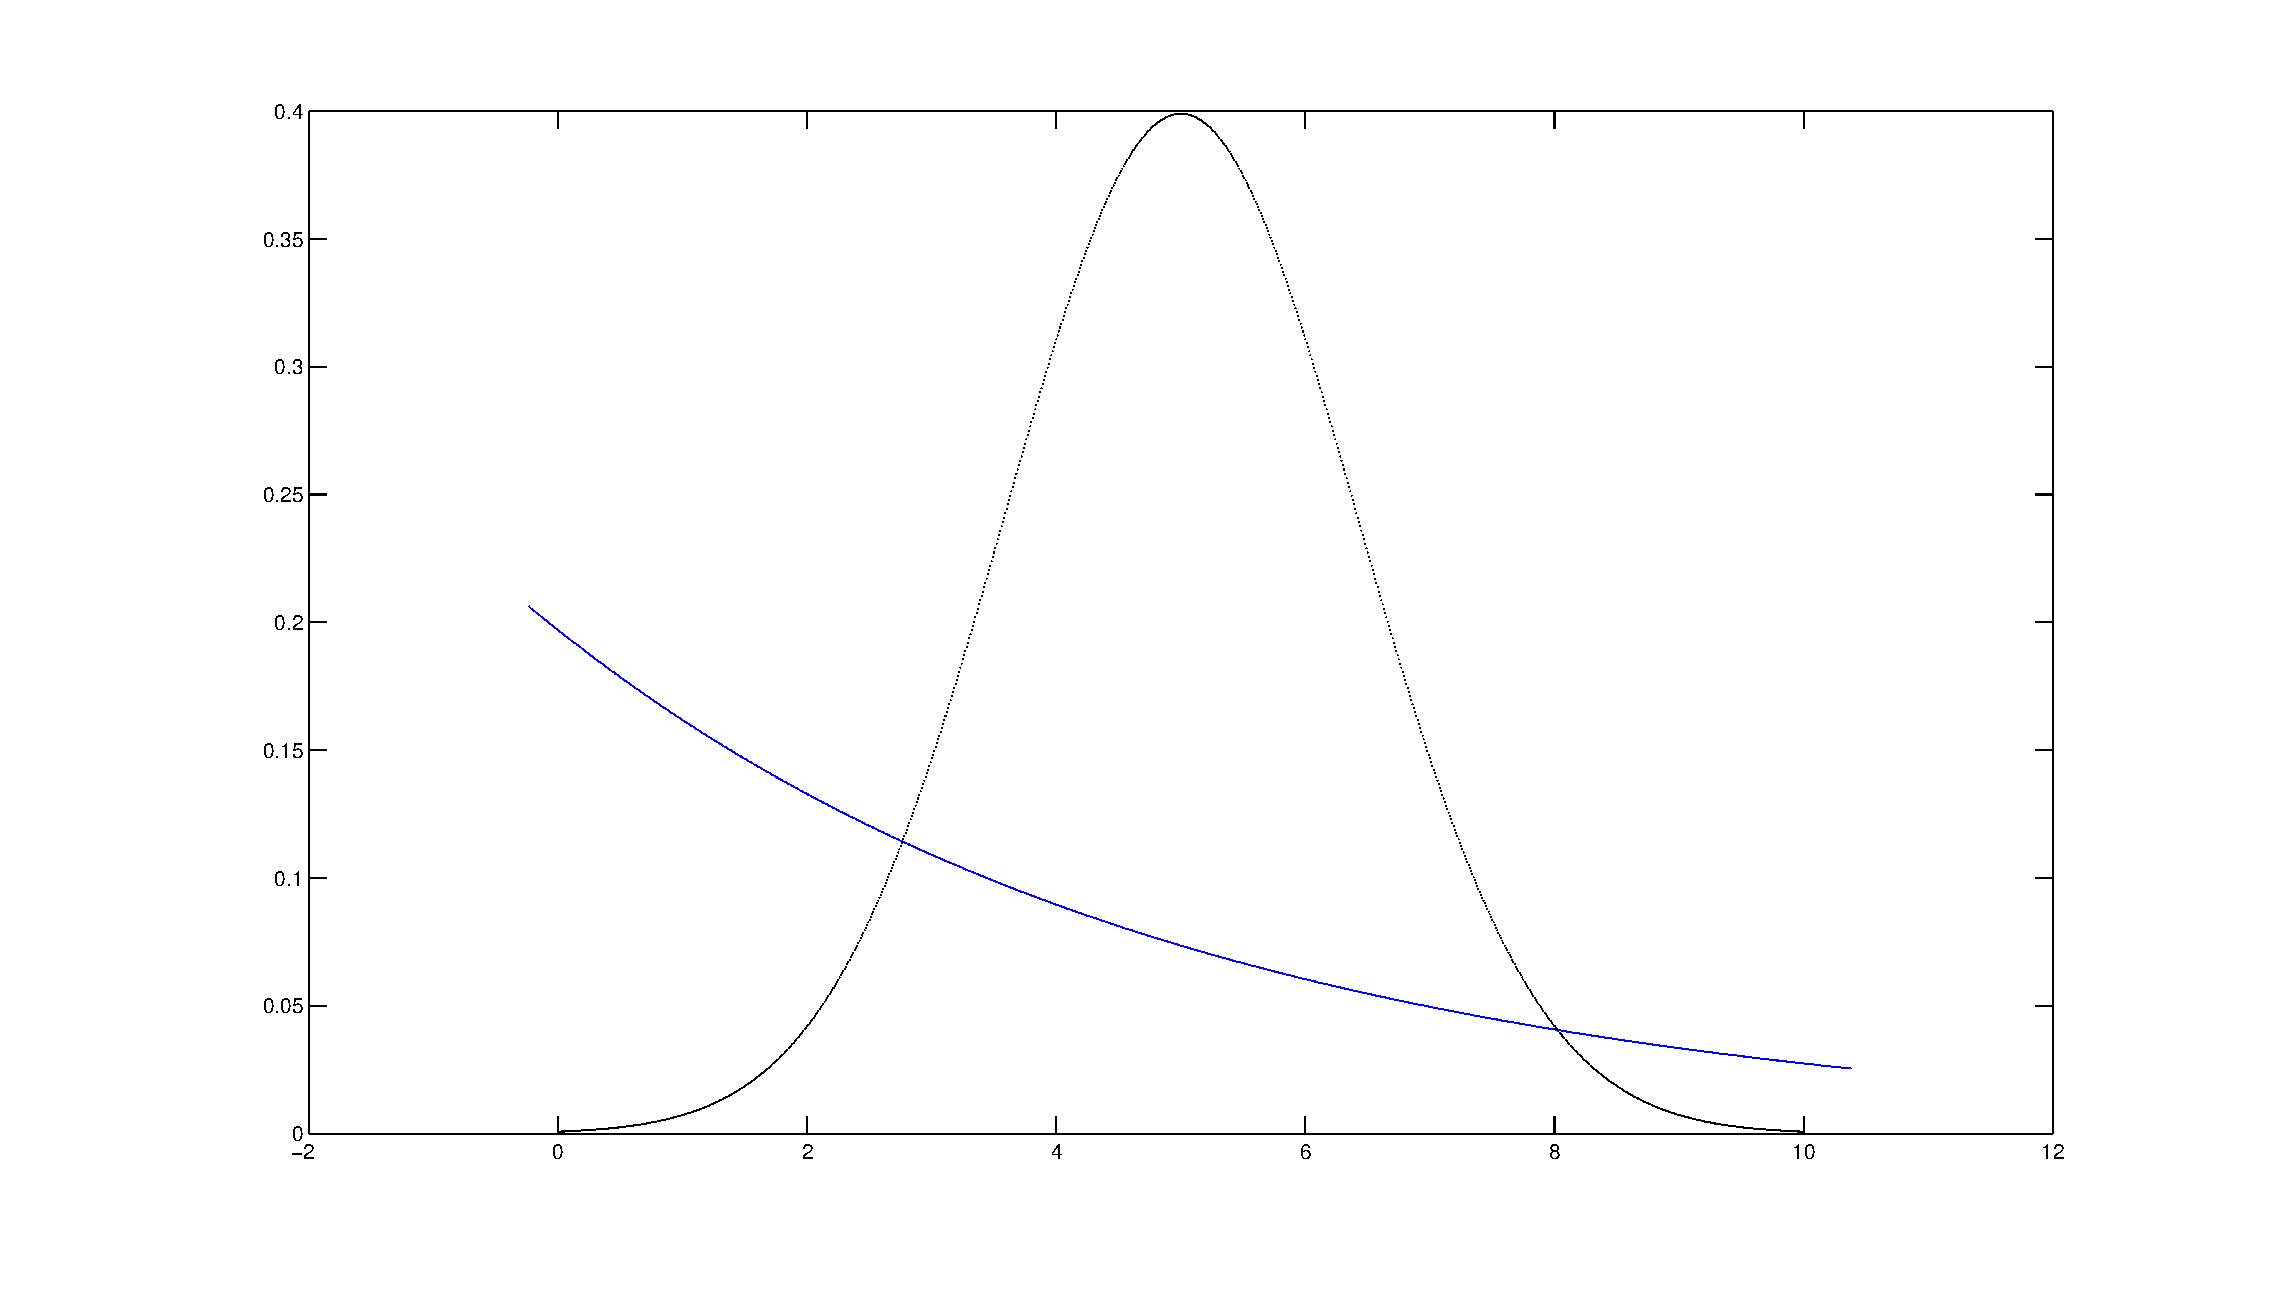
\includegraphics[scale=0.4]{gauss-exp}
\caption{Gaussian sample (black) estimated assuming an exponential PDF (blue)}
\label{fig:ge}
\end{figure}

\begin{figure}
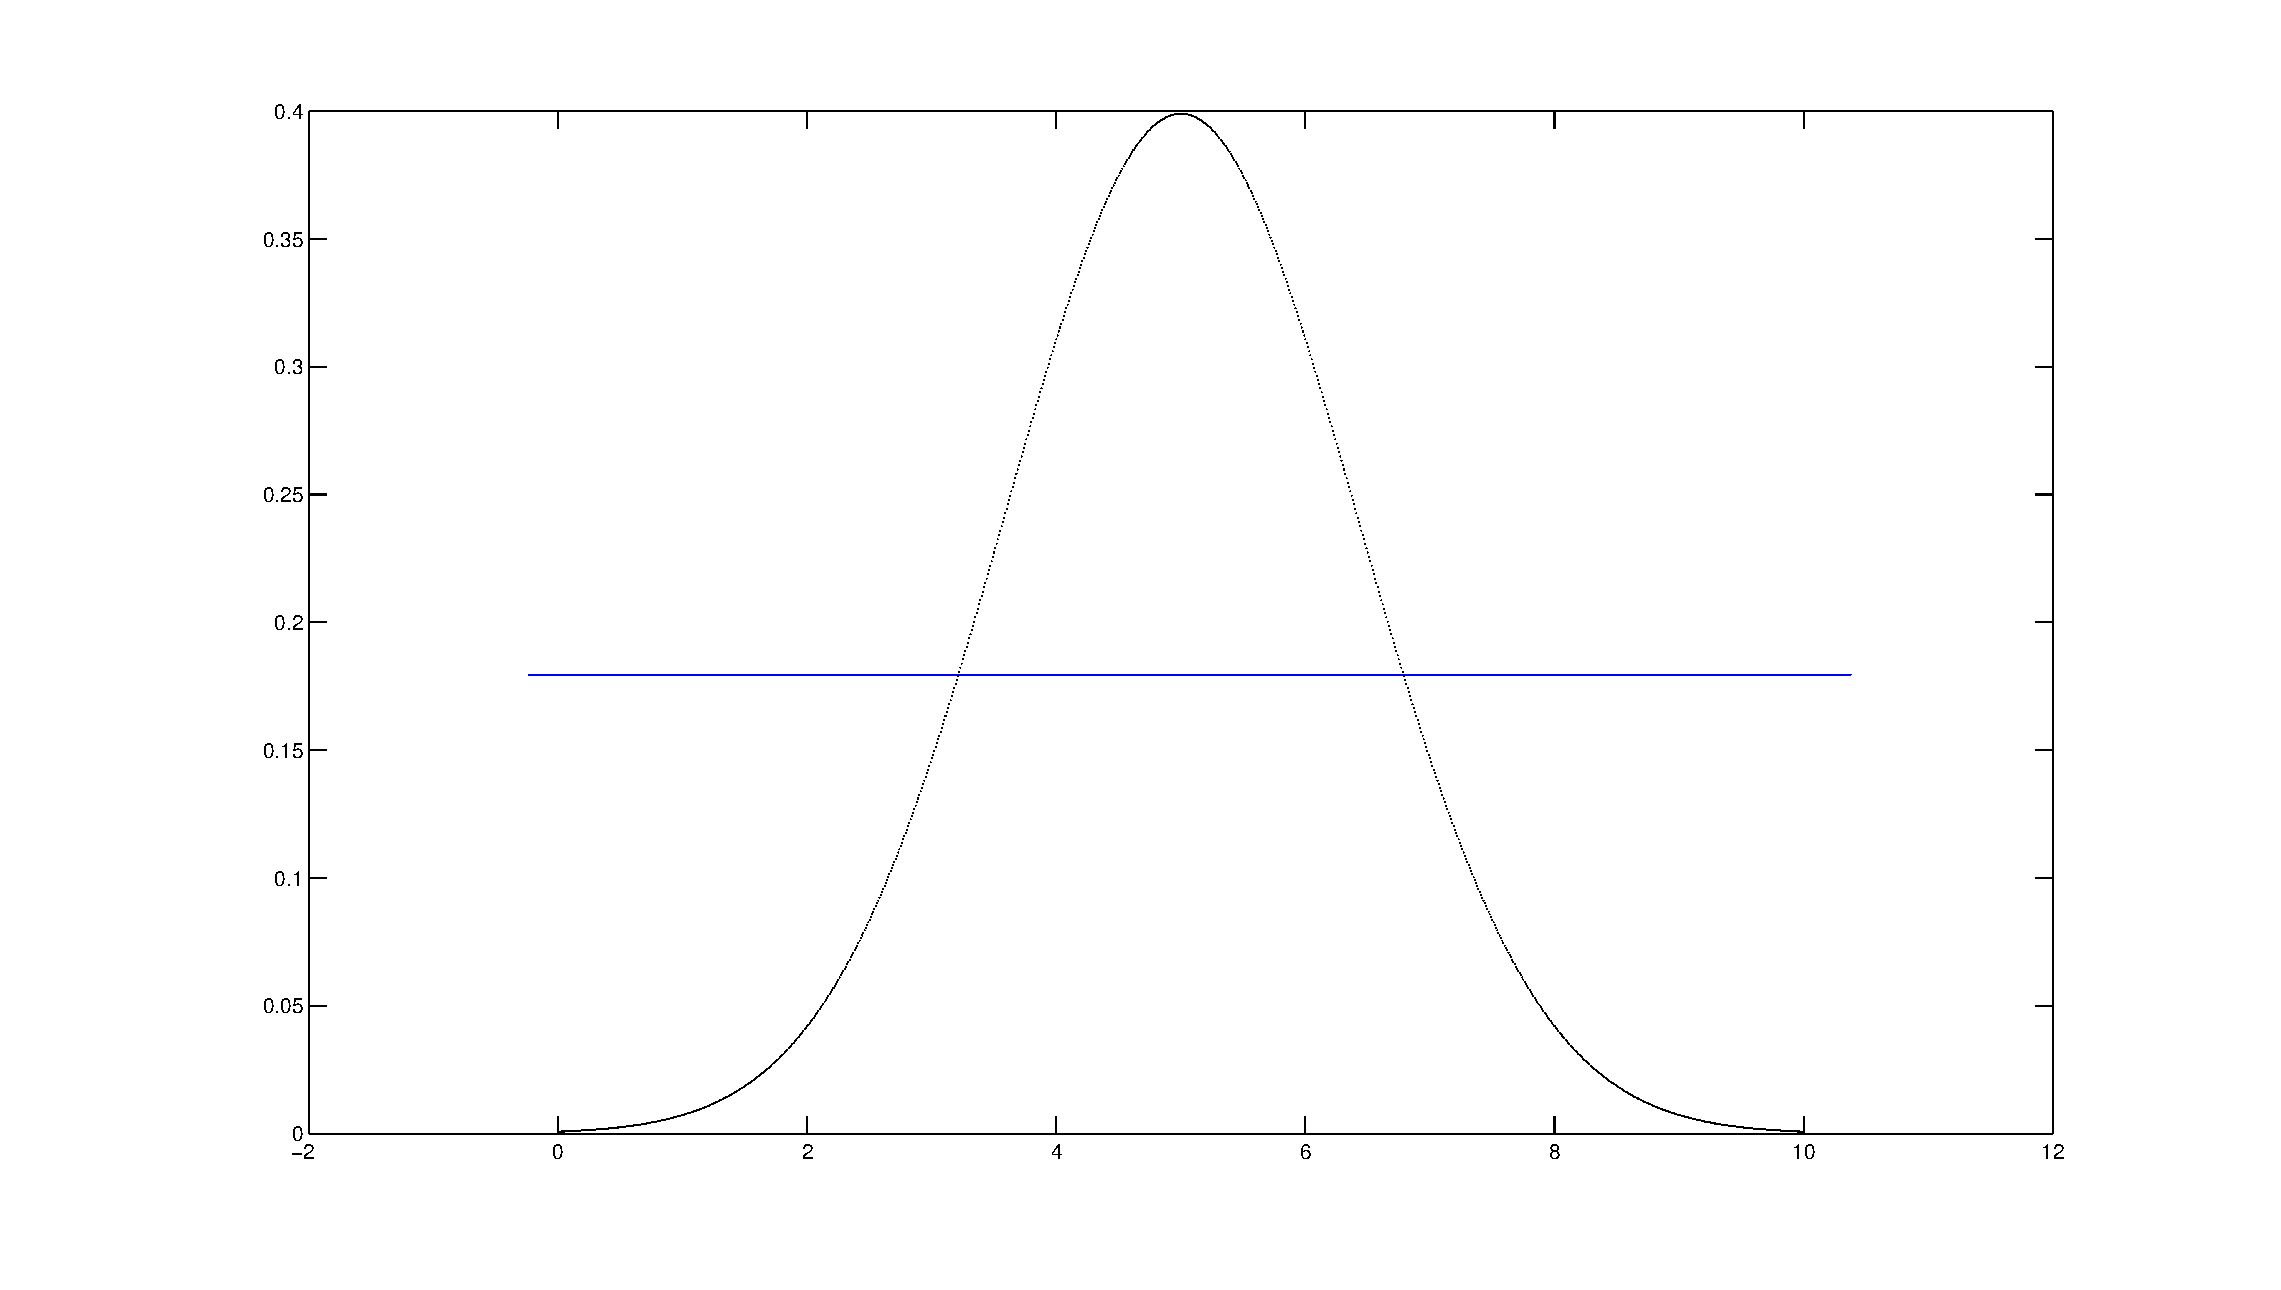
\includegraphics[scale=0.4]{gauss-uni}
\caption{Gaussian sample (black) estimated assuming a uniform PDF (blue)}
\label{fig:gu}
\end{figure}

\begin{figure}
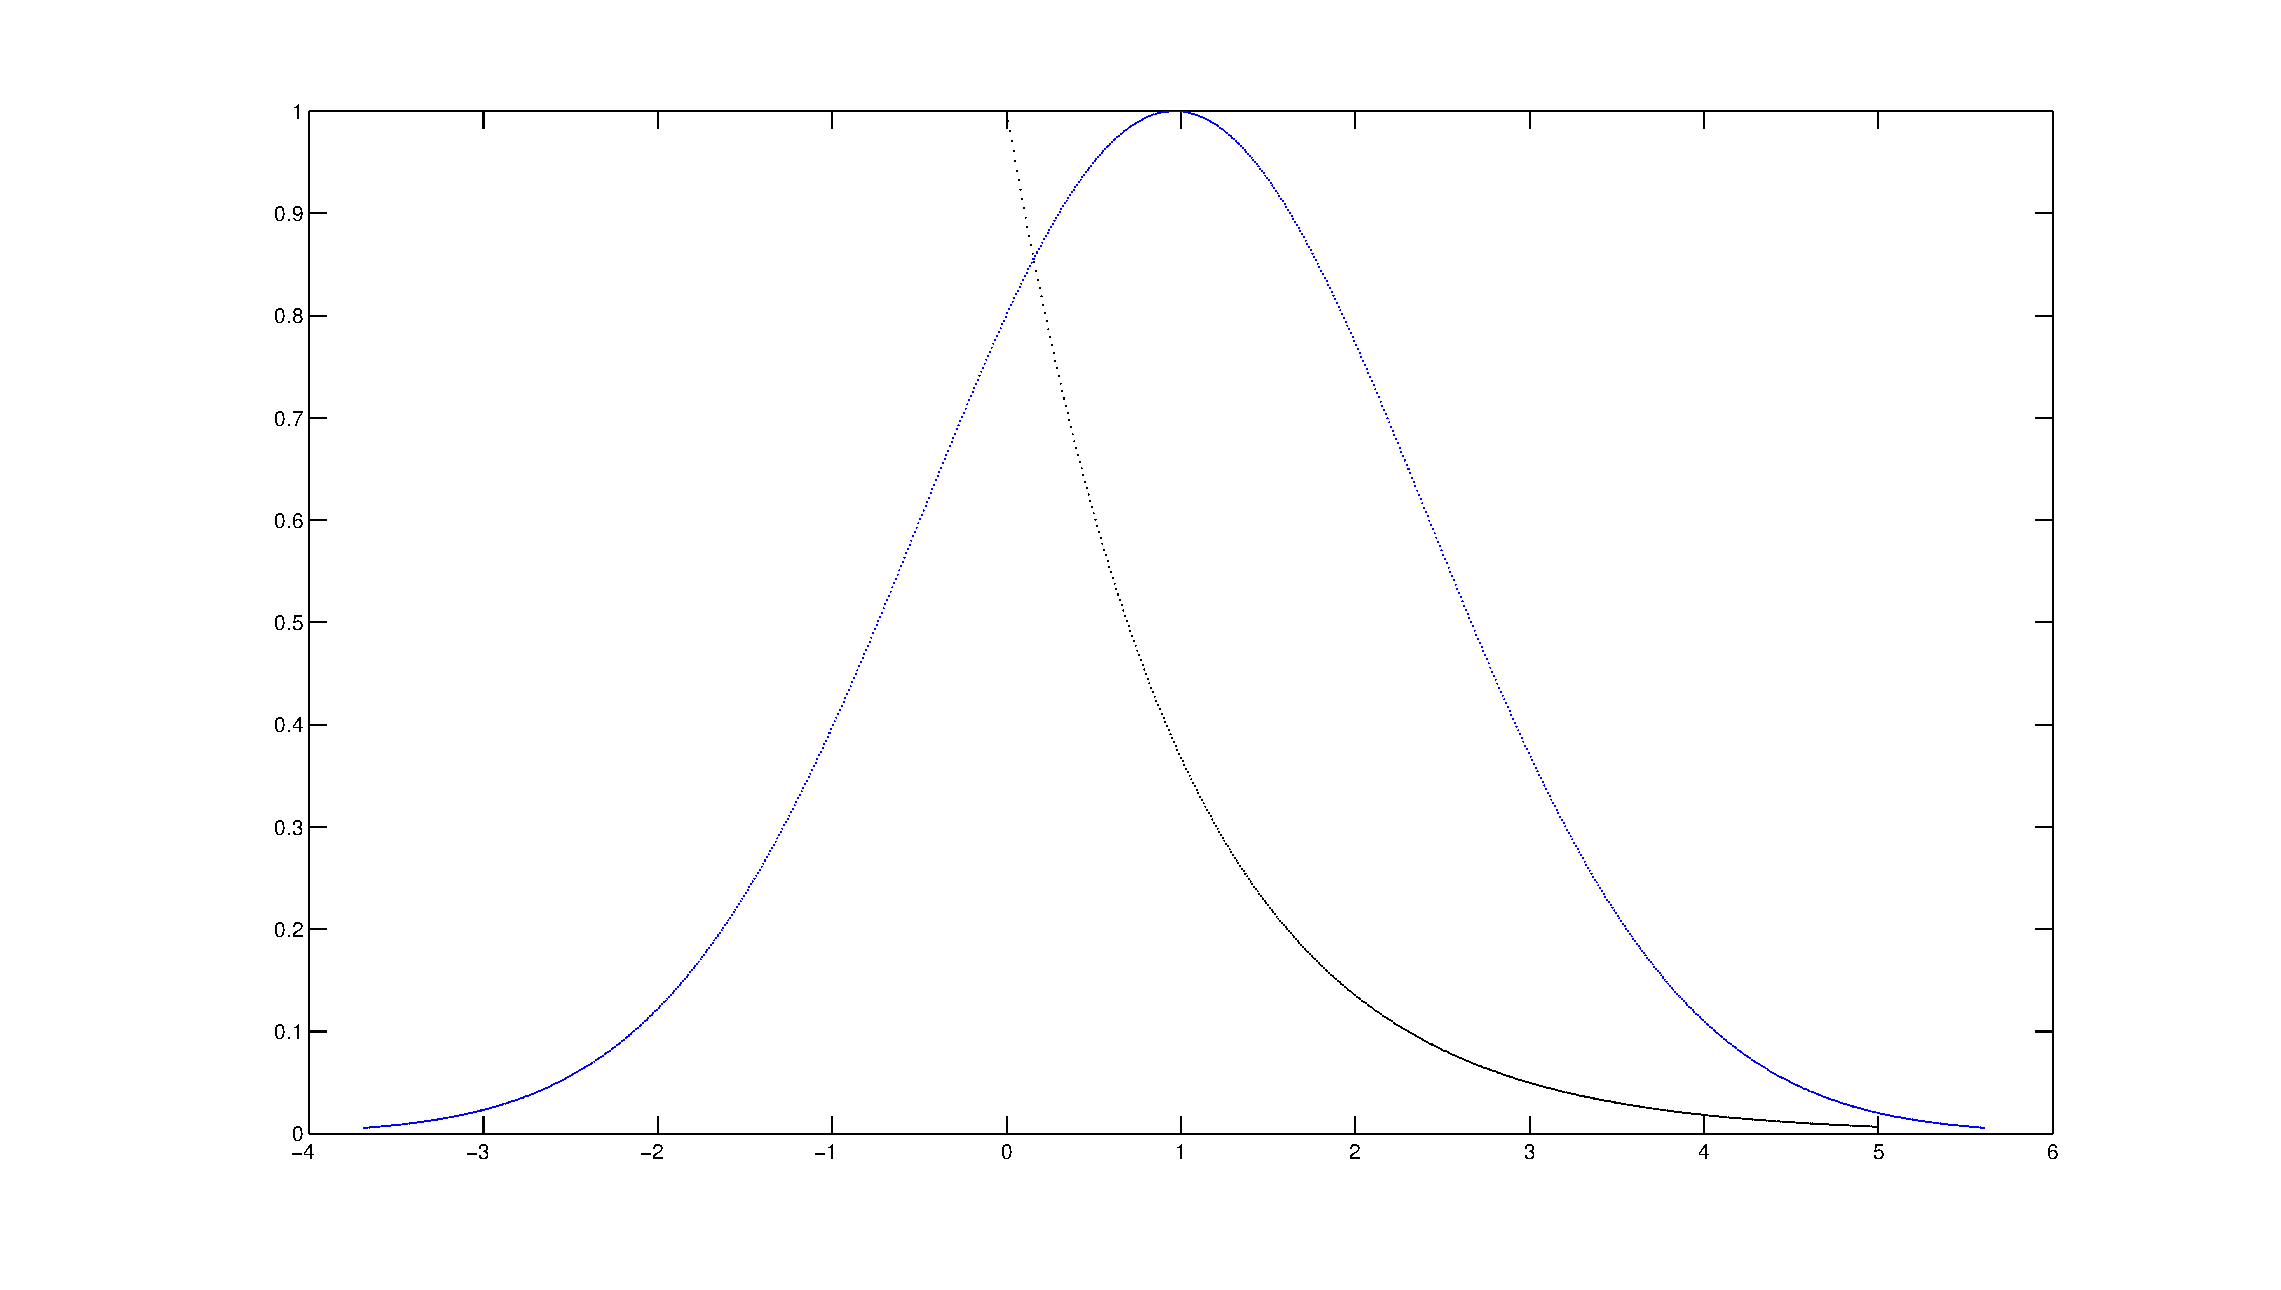
\includegraphics[scale=0.4]{exp-gauss}
\caption{Exponential sample (black) estimated assuming a Gaussian PDF
(blue)}
\label{fig:eg}
\end{figure}

\begin{figure}
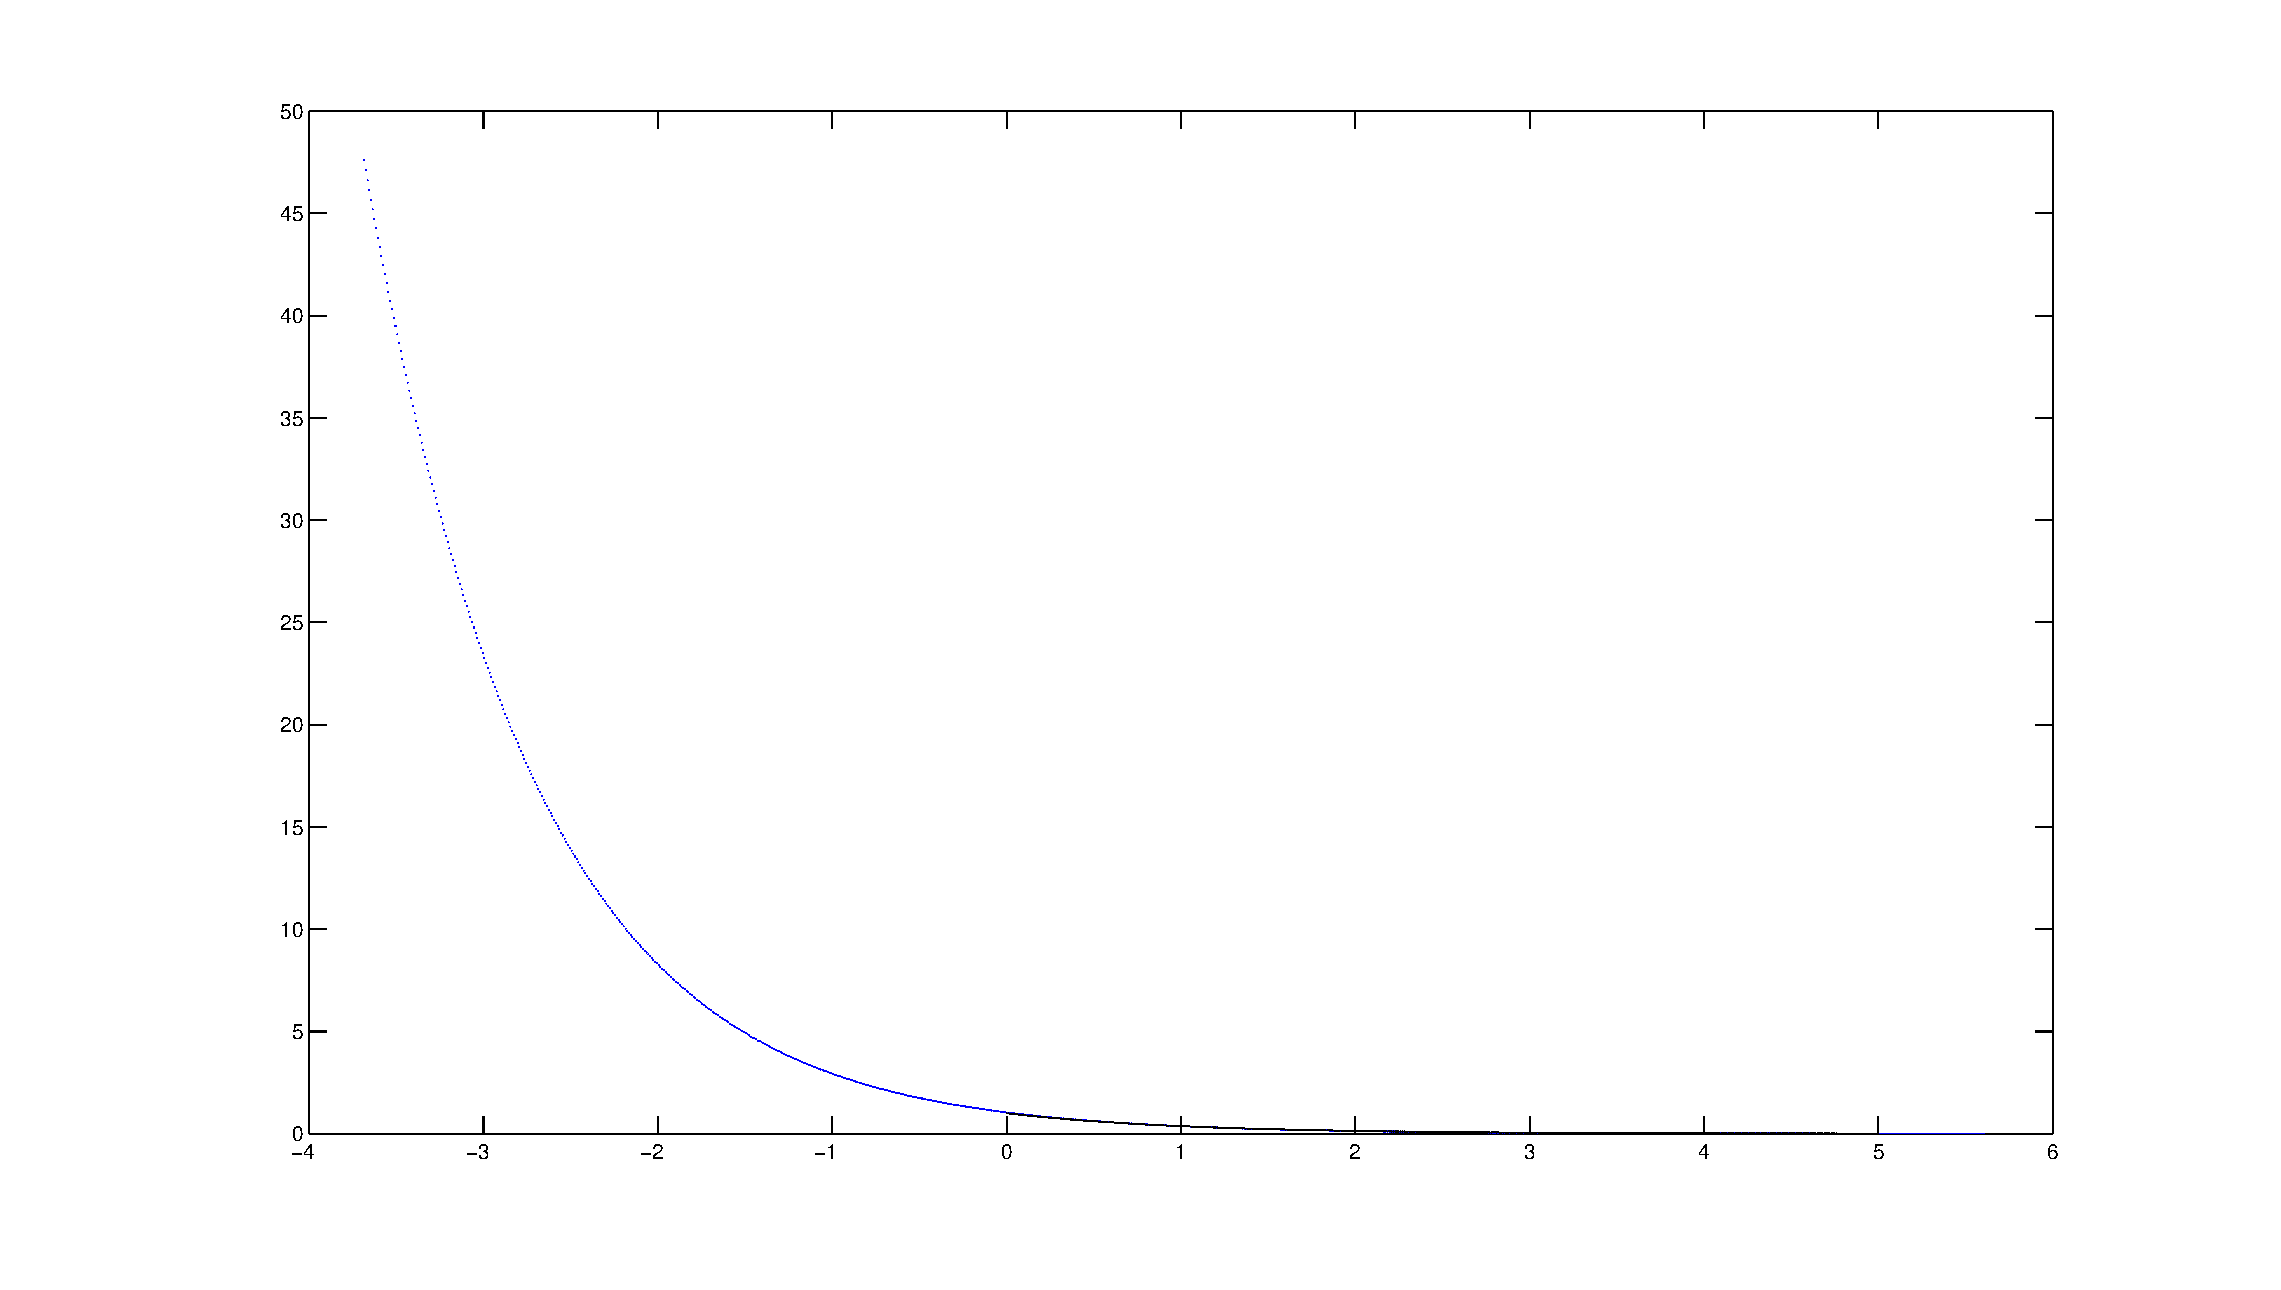
\includegraphics[scale=0.4]{exp-exp}
\caption{Exponential sample (black) estimated assuming an exponential PDF
(blue)}
\label{fig:ee}
\end{figure}

\begin{figure}
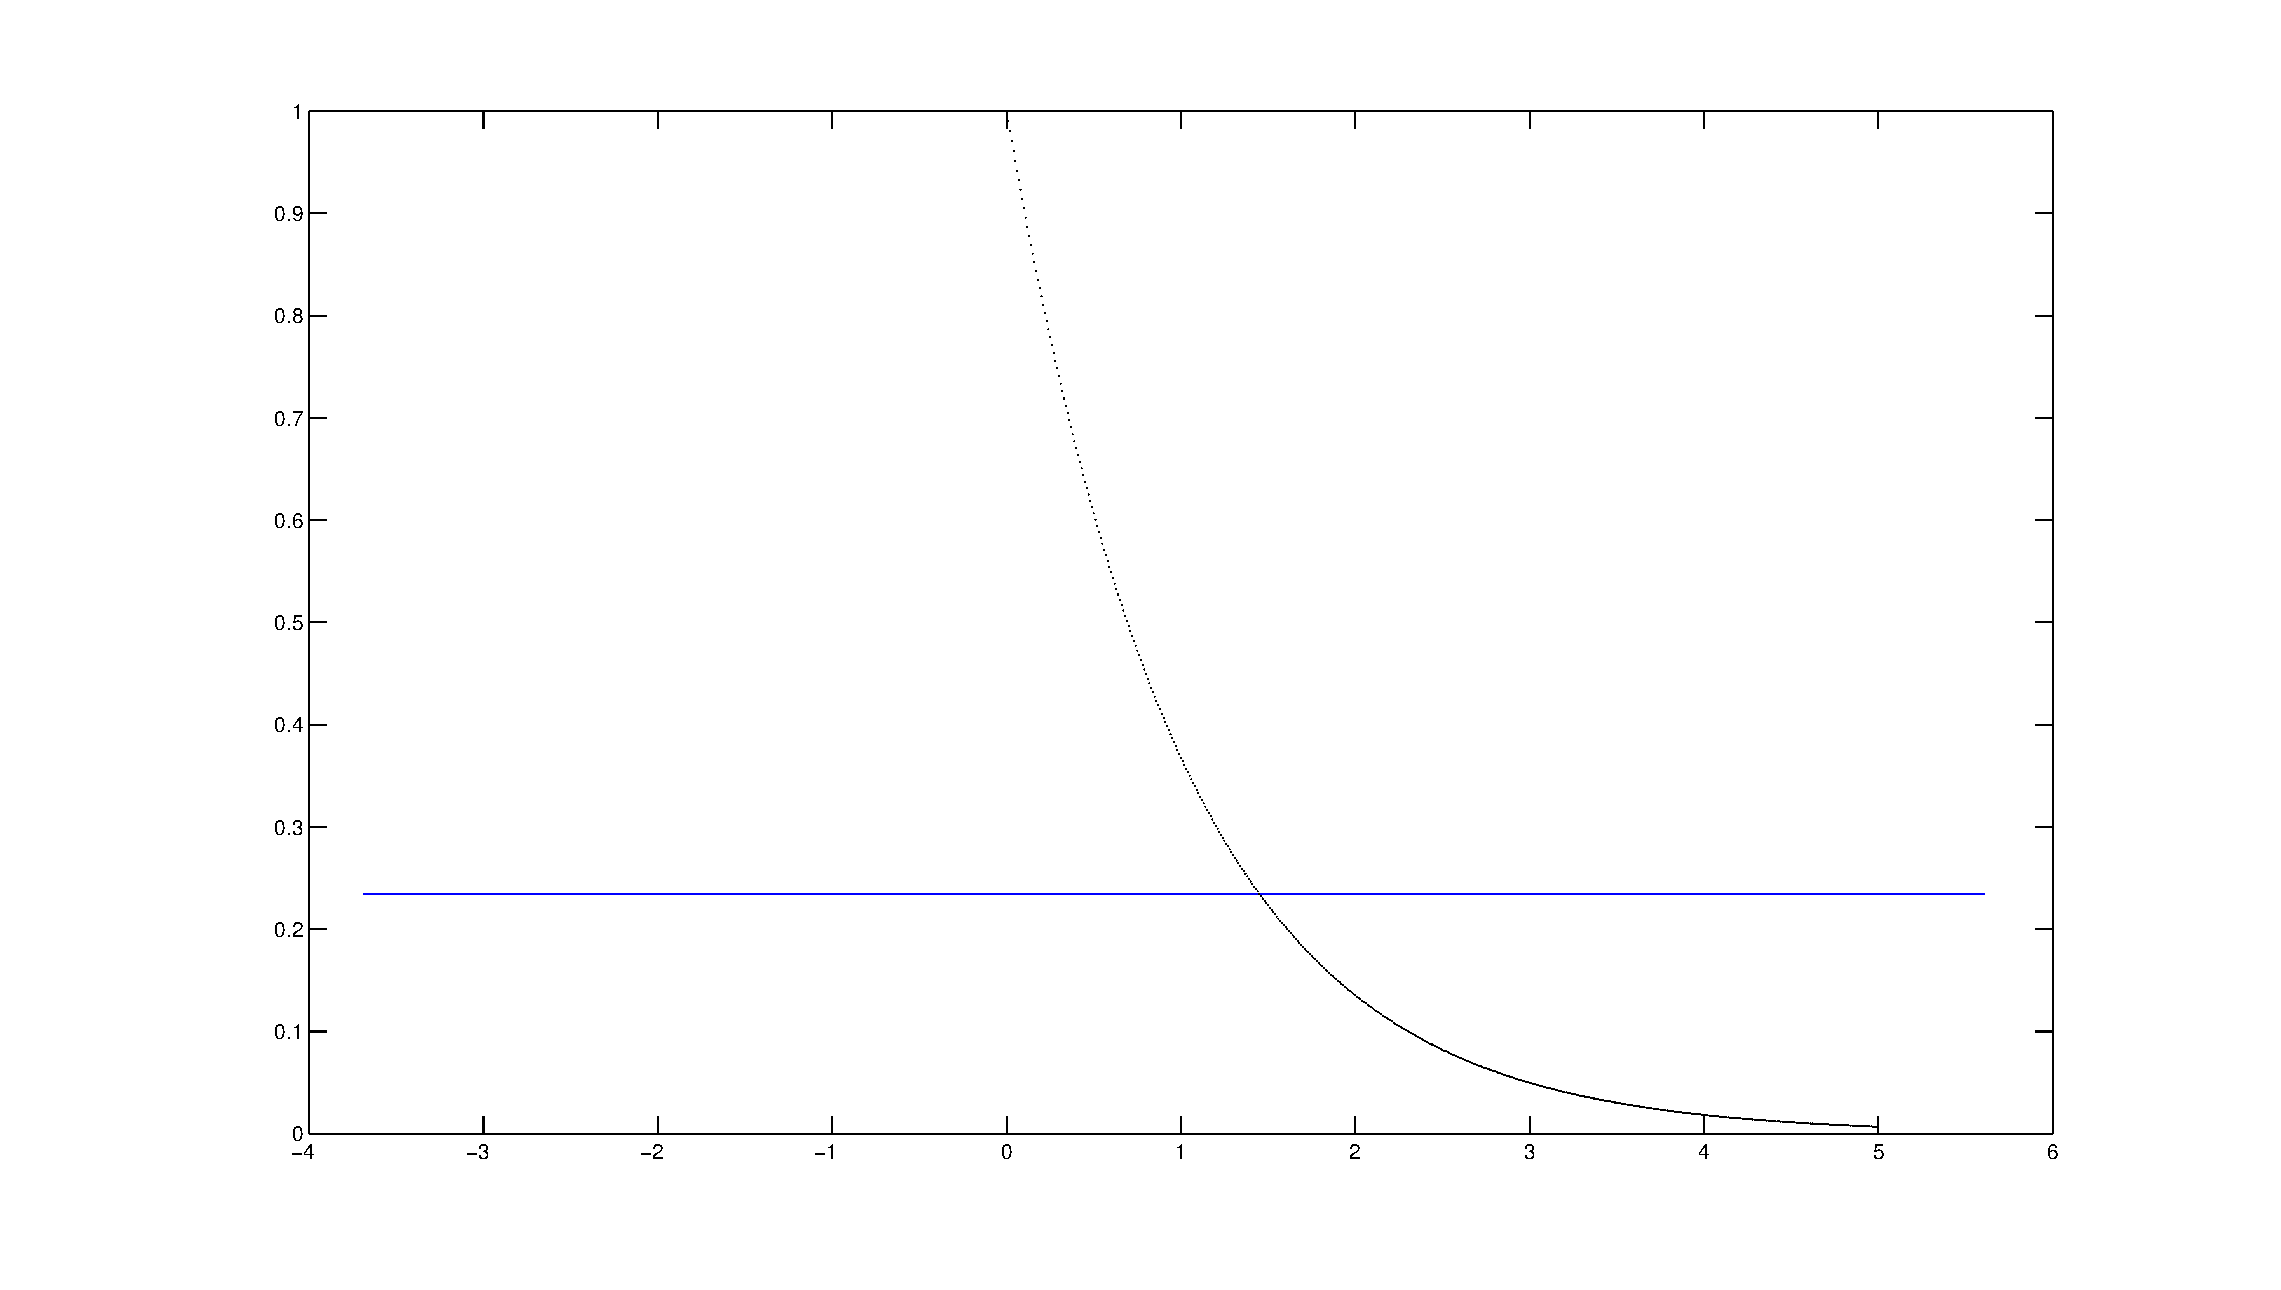
\includegraphics[scale=0.4]{exp-uni}
\caption{Exponential sample (black) estimated assuming a uniform PDF
(blue)}
\label{fig:eu}
\end{figure}

\begin{figure}
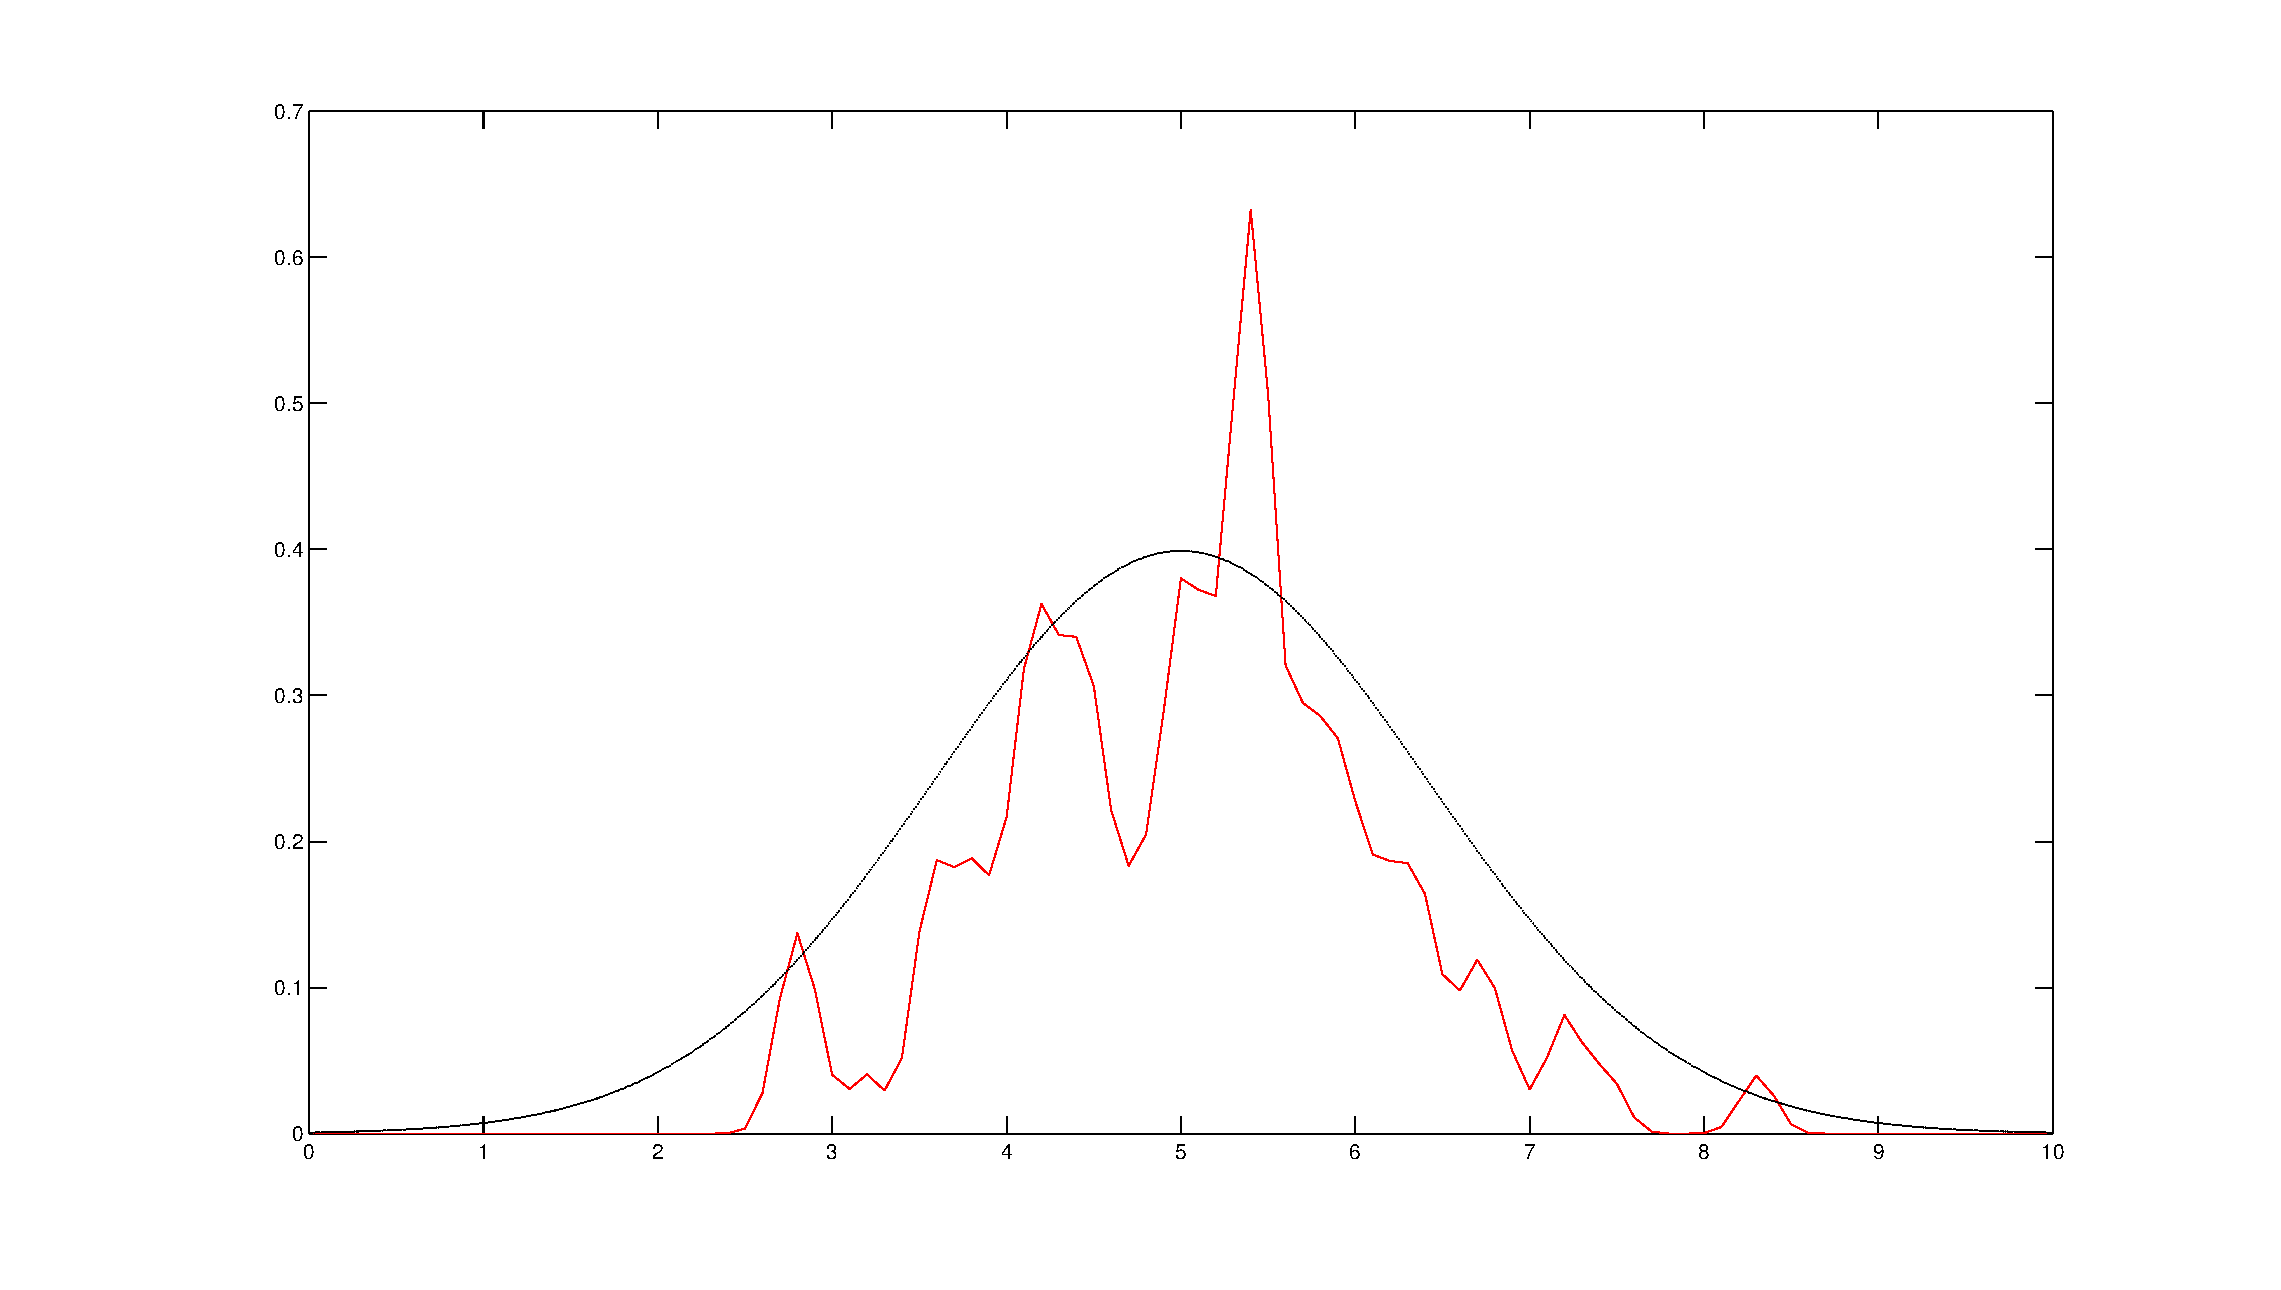
\includegraphics[scale=0.4]{nonpar-parzen-01}
\caption{Gaussian sample (black) estimated using Gaussian Parzen windows
with $\sigma=0.1$ (red)}
\label{fig:parzen1}
\end{figure}

\begin{figure}
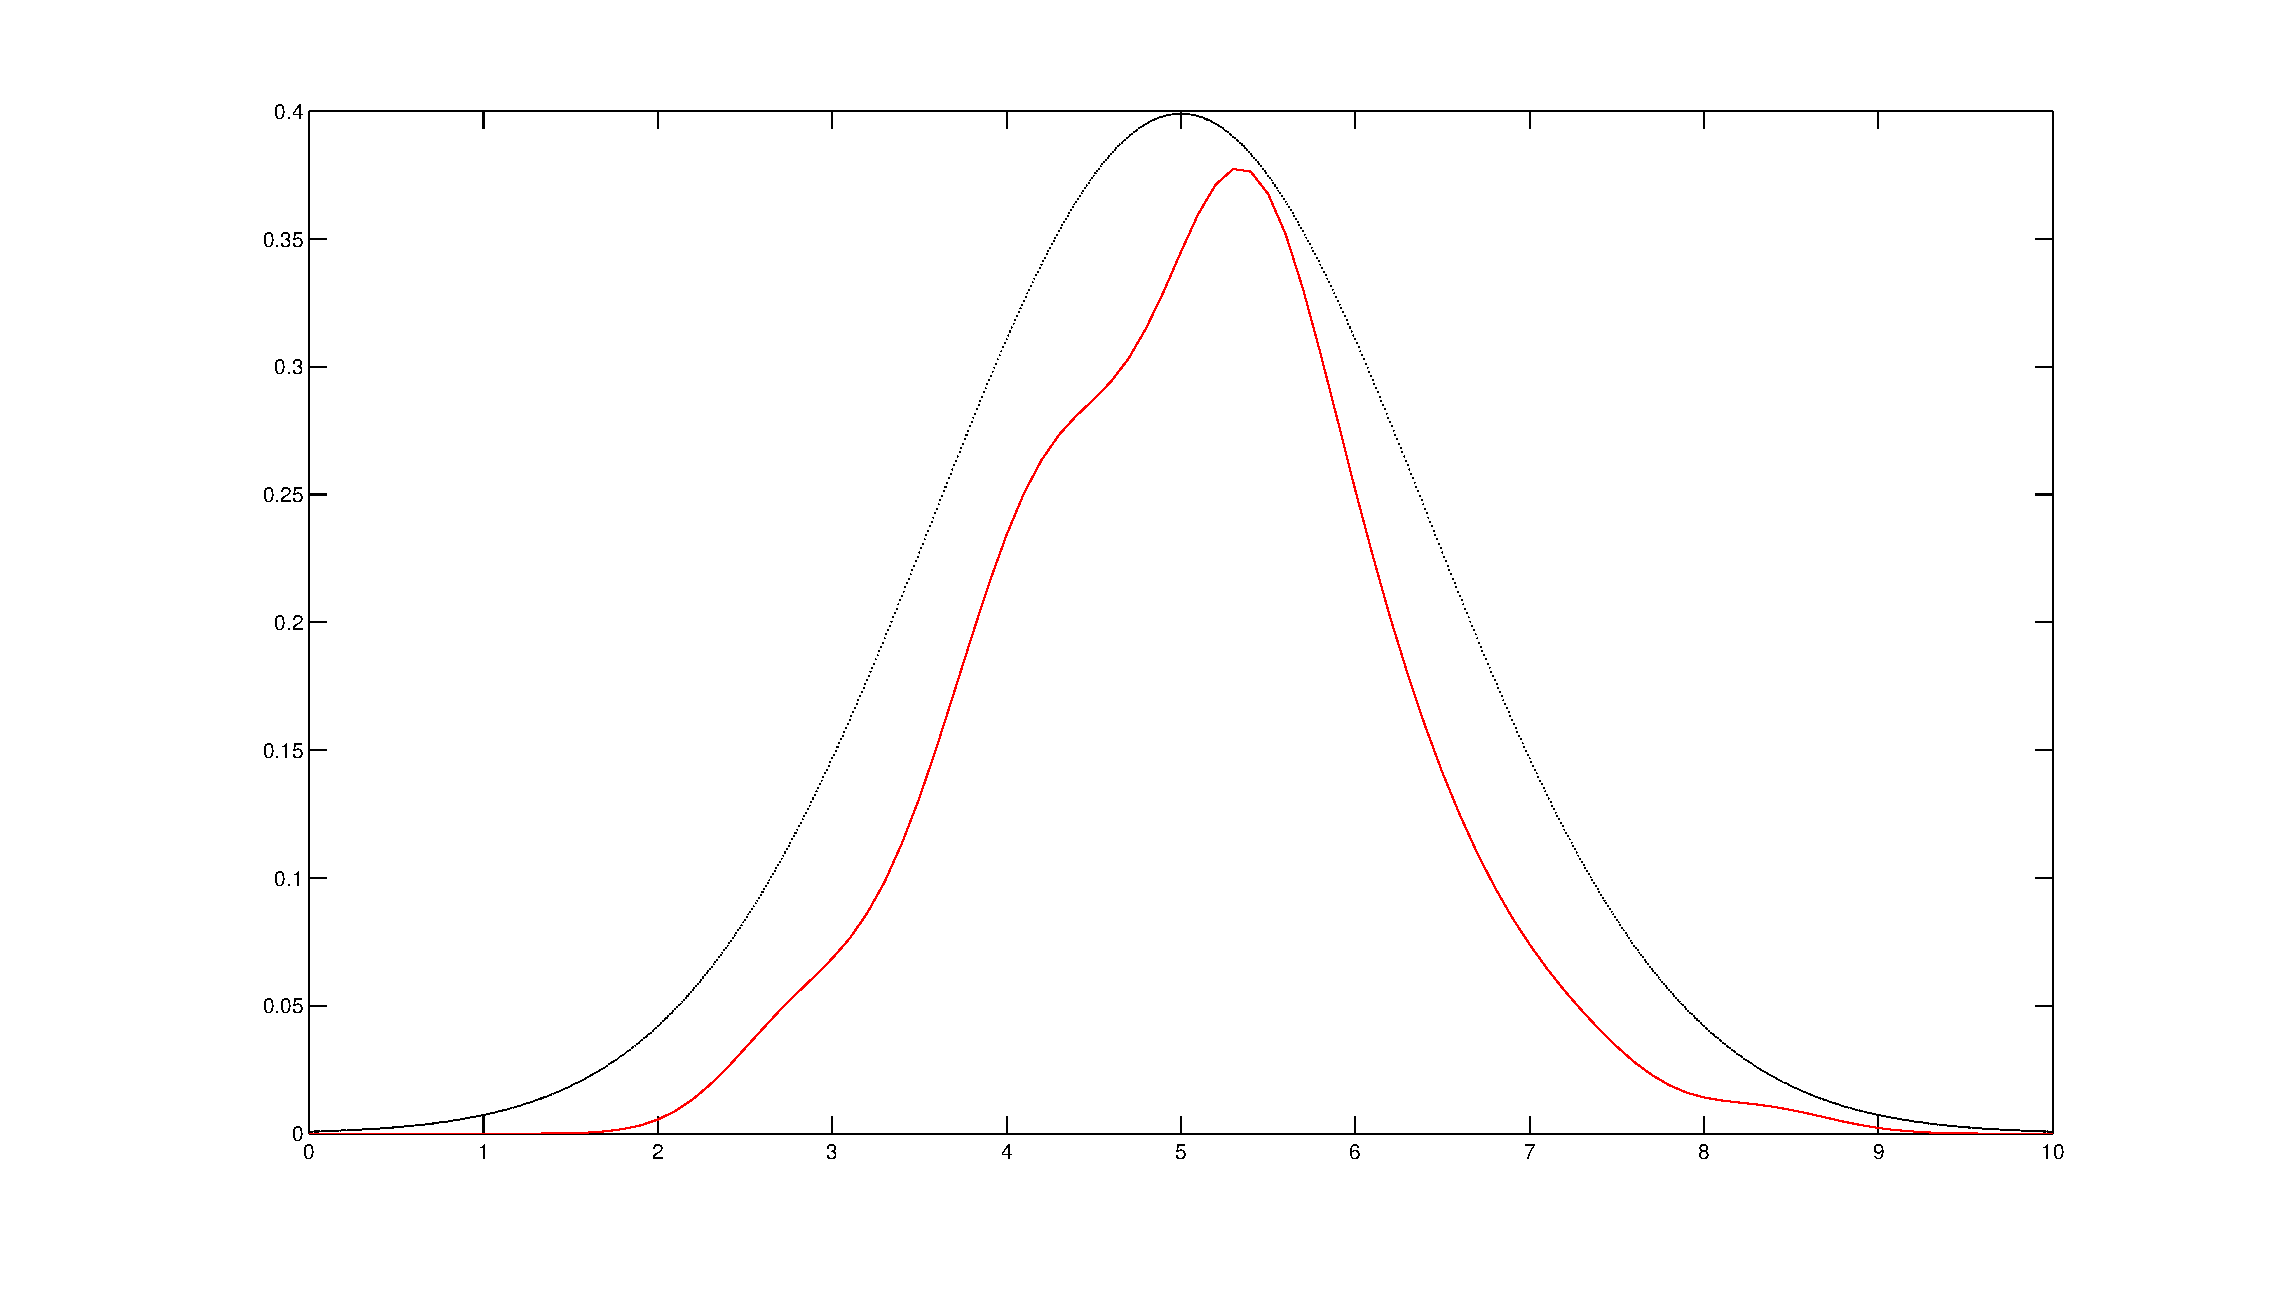
\includegraphics[scale=0.4]{nonpar-parzen-04}
\caption{Gaussian sample (black) estimated using Gaussian Parzen windows
with $\sigma=0.4$ (red)}
\label{fig:parzen4}
\end{figure}